\section{Theoretischer Hintergrund des Versuches}
\label{sec:Theorie}
In den folgenden Abschnitten werden die Grundlagen der Vakuumerzeugung beschrieben
sowie einige wichtige Begriffe definiert. Die Grundlage hierfür ist, wenn nicht anders
angegeben, Pfeiffer Vacuum \cite{pfeiffer}.

\subsection{Das Vakuum}
Der Begriff Vakuum ist definiert als der Zustand eines Gases, wenn der Druck
innerhalb eines Behälters geringer ist als außerhalb oder der Druck geringer
ist als $\SI{300}{\milli\bar}$, was der geringste auf der Erdoberfläche
vorkommende Atmosphärendruck ist. Dieser herrscht auf dem höchsten Punkt der Erdoberfläche,
dem Mount Everest.\\
Das ideale Gasgesetz ist ein Modell, welches ein Gas beschreibt, in dem Gasteilchen
keine Anziehungs- und Abstoßungskräfte aufeinander ausüben. Ebenfalls wird das Volumen
als verschwindend angenommen und ihre Energie nur durch ihre kinetische Energie der Translation
beschrieben. Ideale Gasteilchen stoßen jedoch elastisch mit den Behälterwänden.
Wenn Gase sich im Grenzfall einer verschwindenden Dichte befinden, ist das
ideale Gasgesetz \ref{eqn:idealesGas} eine gute Näherung:
\begin{equation}
 pV = N k_{B} T.
 \label{eqn:idealesGas}
\end{equation}
Hier bezeichnet $V$ das Volumen, $N$ die Teilchenanzahl, $k_{B}$ die
Boltzmann-Konstante, $T$ die Temperatur und $p$ den Druck.
Eine isotherme Zustandsänderung eines solchen idealen Gases kann beschrieben
werden durch das Boyle-Mariottesche Gesetz.
Es besagt, dass bei konstanter Temperatur und konstanter Stoffmenge der Druck direkt
proportional zum Volumen ist:
\begin{align}
  p & \propto \frac{1}{V} & \frac{p}{V} = \text{const}.
  \label{eqn:boylemariotte}
\end{align}
Der Druck ist definiert als eine senkrecht auf eine Fläche $A$ wirkende Kraft $F$:
\begin{equation}
  p = \frac{F}{A}.
  \label{eqn:druck}
\end{equation}
Der Partialdruck hingegen bezeichnet den Druck einer Komponente eines Gasgemischs.
Die Summe aller Partialdrücke ist daher bei idealen Gasen der Totaldruck. Dies
muss bei nicht idealen Gasen nicht notwendigerweise der Fall sein, da die Partialdrücke
sich allgemein gegenseitig stören können.\\
In SI-Einheiten wird der Druck in $\si{\pascal}$ angegeben. Der Zusammenhang zu dem
in Mitteleuropa gebräuchlicheren $\si{\bar}$ ist der Folgende:
\begin{equation}
 \SI{1}{\pascal} = \SI{0.01}{\milli\bar} = \SI{1}{\newton\per\square\meter}.
\end{equation}
Bei sehr geringen Drücken, wie z.B. im Weltall, ist die Angabe eines Drucks nicht
mehr praktikabel; stattdessen wird die Teilchenzahldichte verwendet. Diese gibt an,
wieviele Teilchen sich in einem gegebenen Raumbereich aufhalten.

\subsection{Wichtige Begriffe}
Im folgenden Abschnitt werden wichtige Begriffe im Zusammenhang mit Vakuumapparaturen
erklärt.

\subsubsection*{Die mittlere freie Weglänge}
Als mittlere freie Weglänge wird die Strecke bezeichnet, die ein Gasteilchen
auf geradem Weg im Mittel zwischen zwei Stößen zurücklegen kann. Wenn die Gasteilchendichte
sinkt, steigt die mittlere freie Weglänge an, da sich weniger Teilchen in einem Volumen befinden
und daher die Stoßwahrscheinlichkeit geringer ist. Der Zusammenhang der mittleren freien
Weglänge mit dem Druck unter Annahme des idealen Gasgesetzes ist gegeben durch
\begin{equation}
 \bar{l} = \frac{k_{\text{B}}T}{\sqrt{2}\pi d^{2} p}.
\end{equation}
Hierbei bezeichnet $k_{\text{B}}$ die Boltzmann-Konstante, $T$ die Temperatur, $d$ den
Durchmesser der Gasteilchen und $p$ den herrschenden Druck.

\subsubsection*{Die verschiedenen Vakuums- und Strömungsarten}
Für eine Charakterisierung einer Strömung wird das Verhältnis aus mittlerer
freier Weglänge und dem Durchmesser des Strömungskanals verwendet. Hierfür wird die
Knudsen-Zahl definiert:
\begin{equation}
 K = \frac{\bar{l}}{d}.
\end{equation}
Hierbei bezeichnet $\bar{l}$ die mittlere freie Weglänge und $d$ den Durchmesser
des Strömungskanals. Je nach Größe der Knudsen-Zahl und die Art des Vakuums wird
zwischen Kontinuumsströmung, Knudsenströmung und Molekularer Strömung unterschieden:
\begin{figure}[H]
  \centering
  \includegraphics[scale=0.4]{pictures/strömungen.png}
  \label{fig:strömung}
  \caption{Abbildung der Strömungsarten abhängig von der Knudsen-Zahl \cite{pfeiffer}.}
\end{figure}
\noindent
Hierbei wird zwischen Grobvakuum, Feinvakuum und Hoch- bzw. Ultrahochvakuum unterschieden.
Grobvakuum meint dabei Drücke zwischen $\SI{300}{\milli\bar}$ und $\SI{1}{\milli\bar}$.
Hier finden hauptsächlich Stöße der Gasteilchen untereinander statt, was als Kontinuumsströmung
bezeichnet wird.
Innerhalb der Kontinuumsströmung wird weiter differenziert zwischen der laminaren
und der turbulenten Strömung. Die laminare Strömung wird auch als Schichtströmung
bezeichnet und besteht aus parallel angeordneten Schichten aus Gasteilchen. Durch
Erhöhung der Geschwindigkeit können diese Schichten aufgelöst werden. Dies führt
zu ungeordnet durcheinander laufenden Gasteilchen, was als turbulente Strömung
bezeichnet wird.\\
Innerhalb einer Vakuumapparatur kommt es nur beim schnellen Abpumpen von Atmosphärendruck
sowie bei schnellem Belüften zu turbulenter Strömung. Turbulente Strömung erfordert
höhere Saugvermögen der Vakuumpumpen, weshalb es günstig ist, turbulente Strömung durch
die richtige Dimensionierung der Strömungskanäle zu vermeiden. Um dies sicherzustellen,
reichen bei Grobvakua kleine Leiterdurchmesser, während bei Hoch- und Ultrahochvakua
größere Durchmesser nötig sind, um turbulente Strömung zu verhindern.\\
Das Feinvakuum ist definiert als Druckbereich von $\SI{1}{\milli\bar}$ und $\SI{1e-3}{\milli\bar}$.
Hier ist die mittlere freie Weglänge vergleichbar groß wie der Durchmesser des Strömungskanals,
weshalb die Gasteilchen hauptsächlich mit den Wänden des Gefäßes wechselwirken.
Die Strömung wird als Knudsen-Strömung bezeichnet.
Der Druckbereich von $\SI{1e-3}{\milli\bar}$ bis $\SI{1e-8}{\milli\bar}$ wird als Hochvakuum
bezeichnet. Bereiche darüber werden Ultrahochvakuum genannt. Hier ist die mittlere freie
Weglänge größer als der Durchmesser des Strömungskanals, weshalb hier kaum Wechselwirkungen
der Gasteilchen untereinander stattfindet. Die sich ergebende Strömung heißt molekulare Strömung.

\subsubsection*{Die Absorption und Desorption}
Allgemein bezeichnet die Sorption einen Prozess, der zur Anreicherung eines Stoffes
innerhalb einer Phase oder an der Grenzfläche zwischen zwei Phasen führt.
Die Absorption bezeichnet hierbei die Anreicherung innerhalb einer Phase, während die
Anreicherung zwischen zwei Phasen als Adsoprtion bezeichnet wird. Hierbei meint die Phase
einen räumlichen Bereich, innerhalb dessen die Materialeigenschaften homogen sind.
Handelt es sich nicht um eine Aufnahme, sondern um eine Abnahme, wird von Desorption gesprochen.

\subsubsection*{Reale und virtuelle Lecks}
Als Lecks werden vakuummindernde Prozesse bezeichnet. Ein reales Leck ist eines,
das außerhalb der Vakuumanlage messbar ist, z.B. eine Undichtigkeit. Ein virtuelles
Leck hingegen ist eines, welches nicht außerhalb der Vakuumanlage erkennbar ist.
Beispiele hierfür sind Einschlüsse innerhalb der Anlage, welche nach einer Zeit an
die Materialoberfläche gelangen und austreten.
Eine Quelle von virtuellen Lecks sind die obig erwähnten Desorptionen.

\subsubsection*{Das Saugvermögen einer Vakuumpumpe}
Um den obig erwähnten Lecks entgegenzuwirken, muss die Vakuumpumpe eine Saugvermögen
besitzen, welche mindestens gleich der Leckrate ist. Das Saugvermögen ist definiert
als Volumenänderung pro Zeit:
\begin{equation}
 S = \frac{dV}{dt}.
\end{equation}
Die Bestimmung eines solchen Saugvermögens kann z.B. durch die Aufnahme einer
Evakuierungskurve erfolgen. Dabei handelt es sich um die Druckänderung pro Zeit.

\subsection{Die Methoden der Vakuumerzeugung}

\subsubsection*{Kinetische Pumpen}
Das Funktionsprinzip einer kinetischen Pumpe ist die Beschleunigung der Teilchen in
die Pumprichtung. Eine solche Pumpe benötigt ein Vorvakuum, da bei einer zu hohen
Teilchendichte durch Kollisionen der Teilchen untereinander der Widerstand sehr hoch wird.
Durch ein Vorvakuum kann daher auch der Verschleiß einer solchen Pumpe reduziert werden.
Wenn das Vakuum hingegen schon recht gut ist, funktionieren kinetische Pumpen ebenfalls nicht
ideal, da die mittlere freie Weglänge ab einer gewissen Druckschwelle zu klein ist.
Die Teilchen ändern in diesem Fall ihre Bewegungsrichtung zu früh als dass sie in eine Richtung
beschleunigt werden könnten.

\subsubsection*{Gasfördernde Pumpen}
Nach \ref{eqn:boylemariotte} ist (bei konstanter Temperatur) der Druck
antiproportional zu dem Volumen. Dies wird von gasfördernden Pumpen ausgenutzt,
indem durch Komprimierung und Ausdehnung Druckunterschiede erzeugt werden, welche
bei einem Ausgleichen der Drücke zu Teilchenströmen führen.

\subsubsection*{Gasbindende Vakuumpumpen}
Bei sehr hohen Vakua sind die obig erwähnten Pumpentypen weniger geeignet,
während die gasbindenden Vakuumpumpen hier sinnvoll eingesetzt werden können.
Durch Adsorption können bei einem bereits sehr hohen Vakuum weiterhin effektiv
Gasteilchen gebunden werden. Dies ist weniger effektiv wenn die Teilchenanzahl sehr hoch ist,
in diesem Fall kann nur ein kleiner Teil der Gasteilchen gebunden werden.

\subsection{Die Drehschieberpumpe}
Drehschieberpumpen gehören zu den obig erwähnten gasfördernden Pumpen. Der schematische
Aufbau einer solchen Pumpe ist in Abbildung \ref{fig:drehschieber} gegeben.
\begin{figure}[H]
  \centering
  \caption{Der schematische Aufbau einer Drehschieberpumpe \cite{pfeiffer}.}
  \label{fig:drehschieber}
  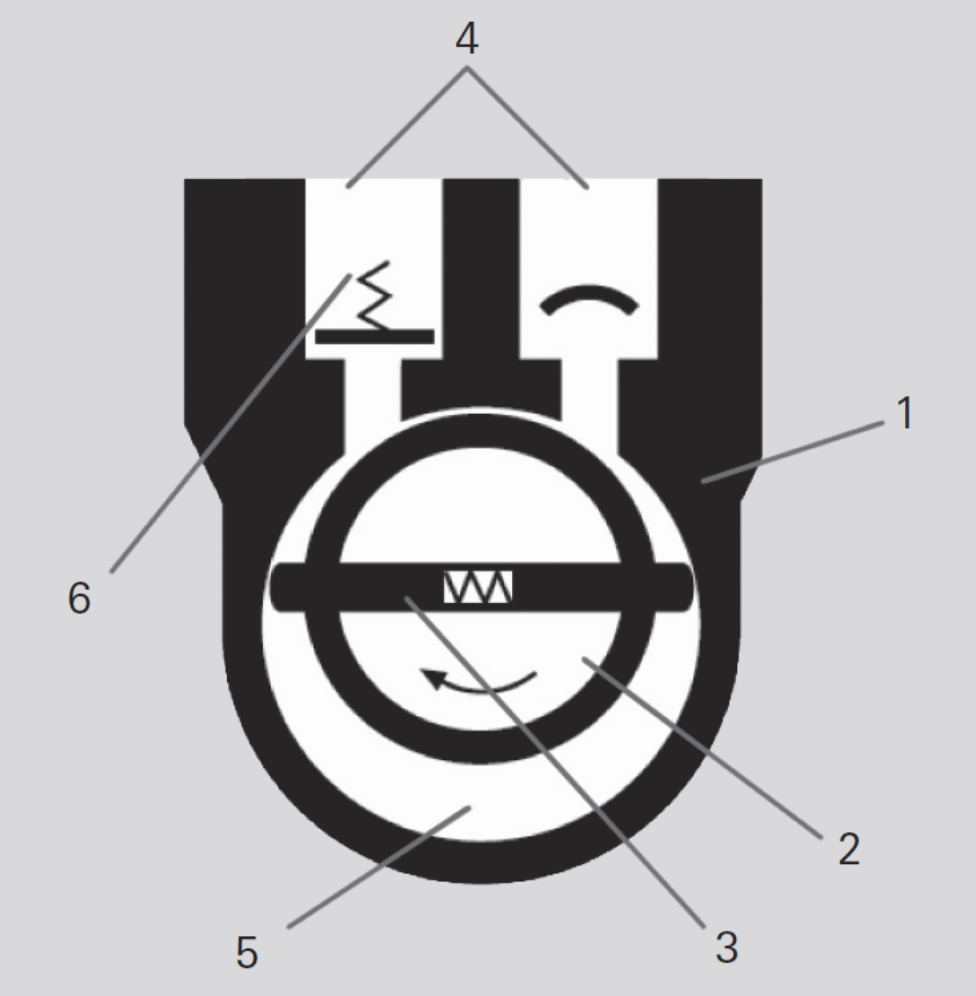
\includegraphics[scale=0.3]{pictures/drehschieber.png}
\end{figure}
\noindent
Der Arbeitsraum [5] einer Drehschieberpumpe wird durch die Schieber [3] des
Rotors [2] aufgeteilt und durch den Stator nach außen abgegrenzt.
Das Einlassventil [4] (rechte Seite) lässt im Betrieb Gas hereinströmen.
Durch Drehen des Rotors [2] vergrößert sich das Volumen des Arbeitsraumes [5], bis der zweite Schieber
das Einlassventil abdeckt. Durch die exzentrische Rotation wird der Arbeitsbereich [5] durch die
weitere Drehung verkleinert, was eine Komprimierung des Gases zur Folge hat. Das Auslassventil [4] (linke Seite)
öffnet sich bei genügend hoher Komprimierung gegen den Atmosphärendruck, was ein Herausströmen des Gases zur
Folge hat. Durch die Ölschmierung des Auslassventils gerät bei jedem Öffnungsprozess eine
kleine Menge Öl in den Arbeitsraum, welches die Schieber gegen den Stator abdichtet. Daher haben
Drehschieberpumpen den Nachteil, dass durch Desorption von Teilchen aus dem verwendeten Schmieröl Lecks
entstehen. Es gibt ein- und
zweistufige Drehschieberpumpen, wobei die zweistufigen Pumpen geringere Drücke erreichen können.
Die in diesem Versuch verwendete zweistufige Drehschieberpumpe erreicht Drücke
von bis zu $p = \SI{2.1 e-2}{\milli\bar}$.

\subsection{Die Turbomolekularpumpe}
Die Turbomolekurlarpumpe gehört zu den kinetischen Pumpen. Eine Turbomolekularpumpe besteht
aus einem Rotor, welcher mit Schaufeln besetzt ist. Zwischen den Rotorschaufeln befinden sich
spiegelsymmetrische Statorschaufeln. Der Rotor dreht sich bei dem in diesem Versuch verwendeten
Exemplar mit bis zu $\SI{1350}{\hertz}$. Die sich drehenden Rotorschaufeln stoßen mit den Gasteilchen,
was eine Beschleunigung der Teilchen in Pumprichtung zur Folge hat. Damit die Gasteilchen so mit den Rotorschaufeln wechselwirken,
muss der Abstand der Rotorschaufeln ähnlich dimensioniert sein wie die mittlere freie Weglänge der
Gasteilchen. In einer Turbomolekularpumpe sollte molekulare Strömung vorliegen, die Teilchen
sollten also fast nicht miteinander und stattdessen hauptsächlich mit dem Rotor wechselwirken.
Der Rotor ist einseitig magnetgelagert, da so eine Verwendung eines Öllagers vermieden werden kann.
Eine Abbildung einer Turbomolekularpumpe ist in \ref{fig:turbomolekular} gegeben.
\begin{figure}
 \centering
 \caption{Eine aufgeschnittene Turbomolekurlarpumpe \cite{turbopumpenbild}. Vertikal verläuft die Achse, auf der die Rotor- und Statorscheiben
 befestigt sind. Oben und unten sind die Lager zu erkennen.}
 \label{fig:turbomolekular}
 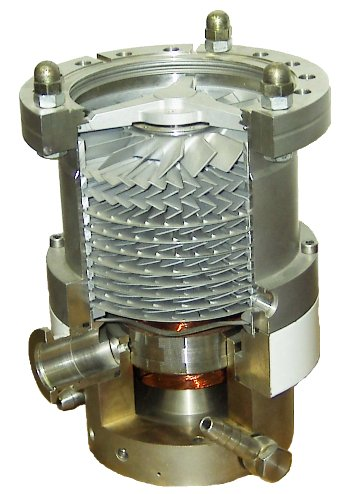
\includegraphics[scale=0.3]{pictures/Cut_through_turbomolecular_pump.jpg}
\end{figure}
\noindent

\subsection{Die Methoden der Vakuummessung}
Die Quantifizierung der Qualität eines Vakuums kann mit einem Vakuummeter durchgeführt werden.
Im Folgenden werden verschiedene Methoden der Vakuummessung beschrieben.

\subsubsection*{Piezo-Vakuummeter}
Ein Piezo-Vakuummeter besteht aus einem Piezo-elektrischen Kristall, welcher bei einem auf ihn wirkenden
Druck eine elektrische Spannung erzeugt. Diese kann gemessen und daraus auf den herrschenden Druck geschlossen
werden. Da der auf den Kristall wirkende Druck antiproportional zu der Vakuumsqualität ist, sinkt der Druck bei
höherer Vakuumqualität ab und kann daher weniger gut gemessen werden. Daher funktioniert ein
Piezo-Vakuummeter am besten im Grobvakuum, da hier die Drücke auf den Kristall höher sind und daher besser
gemessen werden können.
\subsubsection*{Pirani-Vakuummeter}
Das Pirani-Vakuummeter nutzt aus, das (innerhalb eines Druckbereiches von ca. $\SI{1e-4}{\milli\bar}$ bis $\SI{1}{\milli\bar}$)
die Wärmeleitfähgkeit eines Gases druckabhängig ist. Ein in dem zu vermessenden Vakuum befindlicher Draht wird elektrisch geheizt.
Die Wärmeabgabe des Drahtes ist umso höher, desto mehr Gasteilchen die Wärme des Drahtes
aufnehmen können. Der elektrische Widerstand des Drahtes ist abhängig von der Temperatur, weshalb
durch die Widerstandsbestimmung mittels einer Wheatstone-Brücke die Temperatur des Drahtes und darüber der Druck
innerhalb der Kammer ermittelt werden. Wenn andere Formen der Wärmeübertragung (z.B. radiativ durch Wärmestrahlung)
vernachlässigbar sind, kann ein Pirani-Vakuummeter eingesetzt werden. Dies ist im Bereich des Feinvakuums der Fall.

\subsubsection*{Penning-Vakuummeter}
Das Penning-Vakuummeter gehört zu den Kaltionisations-Vakuummetern. Durch elektrische Feldemission werden
Elektronen von einer Kathode freigesetzt und dann auf eine Anode beschleunigt. Auf dem zurückgelegten Weg
ionisieren die Elektronen Gasteilchen, welche dann zur Kathode beschleunigt werden. Aus dem an der Kathode
gemessenen Strom kann auf den Druck geschlossen werden.

\subsubsection*{Bayard-Alpert-Vakuummeter}
Das Bayard-Alpert-Vakuummeter ist ein Heißionisations-Vakuummeter. Die prinzipielle Funktionsweise ähnelt
stark dem Penning-Vakuummeter, mit dem Unterschied dass die Erzeugung der Elektronenemissionen hier auf durch
thermische Emission geschieht.

\subsection{Die Evakuierungskurve}
\label{subsec:evakutheorie}
Die $p(t)$-Kurve wird auch als Evakuierungskurve bezeichnet. Wird von einem idealen Gas ausgegangen,
gilt $p \cdot V = \text{const}$ bei konstanter Temperatur $T$. Durch Ableiten nach der Zeit und nachfolgendes Umstellen ergibt sich:
\begin{equation}
 \frac{\text{d}V}{\text{d}t} = S = - \frac{V}{p} \frac{\text{d}p}{\text{d}t}.
 \label{eqn:evakkrams}
\end{equation}
Für die Lösung der Differentialgleichung \ref{eqn:evakkrams} gilt
\begin{equation}
 p(t) = p_{0} \exp{\frac{-S}{V_{0}}t}.
\end{equation}
Herbei bezeichnet $S$ das Saugvermögen, $V_{0}$ das Volumen der Apparatur, $p_{0}$ den Startdruck und
$t$ die Zeit. Dies beschreibt jedoch keine reale Vakuumpumpe, da eine solche immer durch Lecks und Desorptionen
einen begrenzt niedrigen Enddruck $p_{E}$ besitzt. Dieser Enddruck ist von Null verschieden und kann durch Skalieren
und Verschieben in der Gleichung berücksichtigt werden:
\begin{equation}
 p(t) = (p_{0} - p_{E}) \exp{\frac{-S}{V_{0}}t} + p_{E}.
 \label{eqn:evakuierungskurve}
\end{equation}
Da die Evakuierungskurve \ref{eqn:evakuierungskurve} von dem Saugvermögen $S$ der Vakuumpumpe abhängig ist,
kann durch Messung der Evakuierungskurve das Saugvermögen bestimmt werden. Das Saugvermögen ist jedoch
im allgemeinen keine Konstante, da sie sich für verschiedene Strömungsarten unterscheidet.

\subsection{Definition der Leckrate}
\label{subsec:leckratetheorie}
Das Saugvermögen einer Vakuumpumpe kann nicht nur über die Messung einer Evakuierungskurve, sondern auch
durch eine Leckratenmessung bestimmt werden. Die Leckrate $Q$ ist definiert als das Saugvermögen $S$ geteilt durch
den Gleichgewichtsdruck $p_{G}$:
\begin{equation}
 S = \frac{Q}{p_{G}}.
\end{equation}
Es gilt aber auch
\begin{equation}
 Q = V_{0} \frac{\Delta p}{\Delta t}.
\end{equation}
Daher ergibt sich für das Saugvermögen einer Vakuumpumpe der Ausdruck
\begin{equation}
 S = \frac{V_{0}}{p_{G}} \frac{\Delta p}{\Delta t}.
 \label{eqn:leckratesaugvermögen}
\end{equation}
Durch Variieren der Gleichgewichtsdrücke $p_{G}$ und Bestimmung der Steigung $\frac{\Delta p}{\Delta t}$
kann daher das Saugvermögen einer Vakuumpumpe bestimmt werden. Es muss jedoch ebenfalls beachtet
werden, dass das Saugvermögen durch die restlichen Bestandteile der Apparatur verringert wird und
Gleichung \ref{eqn:leckratesaugvermögen} eine Idealisierung darstellt. Die Reduzierung des idealen
Saugvermögens $S_{\text{Ideal}}$ durch die Apparatur wird durch den Leitwert $L$ beschrieben. Das reale Saugvermögen
berechnet sich dann nach
\begin{equation}
 S_{\text{Effektiv}} = \frac{S_{\text{Ideal}} \cdot L}{S_{\text{Ideal}} + L}.
 \label{eqn:saugvermögenleitwert}
\end{equation}
Der Leitwert beschreibt hierbei die Strömungswiderstände innerhalb der Apparatur, welche durch Reibung der
Gasteilchen untereinander und mit den Wänden hervorgerufen werden.

\section{Berechnung der Unsicherheiten}
\label{sec:unsicherheiten}
Bei den obig beschriebenen Messungen der Evakuierungskurve und der Leckrate handelt es sich
im allgemeinen um Messwerte, welche mit einer Unsicherheit behaftet sind. In den in der
Auswertung durchgeführten Berechnungen müssen diese beachtet werden. Messungenauigkeiten
pflanzen sich in Berechnungen nach der Gaußschen Fehlerfortpflanzung fort. Für den Fall mehrerer
nicht-korrelierter Unsicherheiten ist die resultierende Unsicherheit durch Gleichung \ref{eqn:gaußfort}
gegeben.
\begin{equation}
  \Delta f = \sqrt{\sum_{i=1}^{n} \left( \frac{\partial f}{\partial x_{i}} \Delta x_{i} \right)^{2}}
 \label{eqn:gaußfort}
\end{equation}
Durch Anwenden der Gleichung \ref{eqn:gaußfort} ergibt sich für den Fehler der logarithmischen Fits
\begin{equation}
  \sigma_{log} = \sqrt{\frac{\sigma_p^2}{(p-p_E)^2}+\frac{\sigma_{p_{0}}^2}{(p_0-p_E)^2}+\sigma_{p_E}^2 \left(\frac{1}{p_0-p_E}-\frac{1}{p-p_E}\right)^2}.
  \label{eqn:fehlerlog}
\end{equation}
Hierbei beschreiben $\sigma_{p}$, $\sigma_{p_{0}}$ sowie $\sigma_{p_{E}}$ die Unsicherheit der jeweiligen Größe.
Für die Unsicherheiten der Saugvermögensberechnung und der Berechnung des Leitwertes ergibt sich nach
\ref{eqn:gaußfort} jeweils
\begin{align}
  \sigma_{S} = & \sqrt{\left(\frac{m^2}{p_g^2}\right) \cdot \sigma_{V}^2 + \left(\frac{V^2}{p_g^2}\right) \cdot \sigma_m^2 + \left(\frac{m^2 V^2}{p_g^4}\right) \cdot \sigma_p^2} \\
  \sigma_{L} = & \sqrt{\left( \frac{ S_{\text{Ideal}}^2}{(S_{\text{Effektiv}}- S_{\text{Ideal}})^2} \right) \cdot \sigma_{S_{\text{Effektiv}}}^2 + \left( \frac{S_{\text{Effektiv}}^2}{(S_{\text{Effektiv}}- S_{\text{Ideal}})^2} \right) \cdot \sigma_{S_{\text{Ideal}}}^2} \quad.
  \label{eqn:fehlersaugleit}
\end{align}
Hier bezeichnen $\sigma_{m}$ und $\sigma_{V}$ die Unsicherheit der jeweiligen Größe.
Bei der Berechnung der arithmetischen Mittelwerte ergibt sich für die Unsicherheit der resultierenden
Größen $\Delta x$
\begin{equation}
 \Delta x = \sqrt{\frac{1}{n(n-1)} \sum_{i=1}^{n} (\bar{x} - x_{i})^{2}}.
 \label{eqn:statfehler}
\end{equation}
Hierbei bezeichnet $n$ die Anzahl der (nicht-korrelierten) Messwerte, $\bar{x}$ den arithmetischen Mittelwert
und $x$ den jeweiligen Messwert. Die Berechnung der Unsicherheiten wird mithilfe des Paketes
\textit{Uncertainties}\cite{uncertainties}
der Sprache \textit{Python}\cite{python} durchgeführt.

\subsection{Ungenauigkeiten der verwendeten Geräte}
\label{subsec:ungenauigkeiten}
Die verwendeten Vakuummeter Pfeiffer Vacuum PKR 360 haben in dem Messbereich von $\SI{1e-8}{\milli\bar}$ bis
$\SI{100}{\milli\bar}$ eine Messungenauigkeit von $\SI{30}{\percent}$ des jeweiligen Messwertes.
Das Vakuummeter Pfeiffer Vacuum TPG202 besitzt eine Messunsicherheit von $\SI{0.3}{\percent}$
des Vollausschlages in einem Messbereich von $\SI{1200}{\milli\bar}$ bis $\SI{10}{\milli\bar}$
sowie $\SI{10}{\percent}$ des Messwertes in einem Messbereich von $\SI{10}{\milli\bar}$ bis
$\SI{2e-3}{\milli\bar}$.
